\documentclass[12pt, a4paper]{article}

\usepackage[T1]{fontenc}
\usepackage[utf8]{inputenc}
\usepackage[charter, cal=cmcal]{mathdesign}
\usepackage[scaled=0.92]{helvet}
\usepackage{geometry}
\geometry{a4paper, top=30mm, bottom=30mm, inner=30mm, outer=30mm}

\usepackage{amsmath, amsthm}
\usepackage{amssymb}
\usepackage{xcolor}
\usepackage{tikz}
\usetikzlibrary{arrows.meta, calc}
\usepackage{fancyhdr}
\usepackage{titlesec}
\usepackage{enumitem}
\usepackage{booktabs}
\usepackage{array}
\usepackage{parskip}
\usepackage[colorlinks=true, linkcolor=NavyBlue, urlcolor=NavyBlue, citecolor=NavyBlue]{hyperref}

% ── Colours (Journey 6 — navy blue / gold) ────────────────────────────────────
\definecolor{NavyBlue}{HTML}{1E3A8A}
\definecolor{ModuleColor}{HTML}{2563EB}
\definecolor{PuzzleColor}{HTML}{D97706}
\definecolor{DiscoveryColor}{HTML}{B45309}
\definecolor{ProblemColor}{HTML}{6B21A8}
\definecolor{ReflectColor}{HTML}{0D9488}
\definecolor{LightBlue}{HTML}{EFF6FF}
\definecolor{LightGold}{HTML}{FEF3C7}
\definecolor{LightGreen}{HTML}{ECFDF5}

% ── Custom Environments (No TColorBox for Math style) ─────────────────────────
\newenvironment{puzzlebox}
  {\par\medskip\fillcolorbox{LightGold}{PuzzleColor}{The Puzzle}}
  {\par\medskip}

\newenvironment{discoverybox}
  {\par\medskip\fillcolorbox{LightGreen}{DiscoveryColor}{Discovery}}
  {\par\medskip}

\newenvironment{namedconcept}[1]
  {\par\medskip\fillcolorbox{LightBlue}{NavyBlue}{#1}}
  {\par\medskip}

\newenvironment{reflectionbox}
  {\par\medskip\fillcolorbox{LightBlue}{ReflectColor}{Reflection}}
  {\par\medskip}

\newcommand{\fillcolorbox}[3]{%
  \noindent
  \filldrawbox{#1}{#2}{\textbf{\sffamily\color{white}#3}}\par\nobreak\vspace{4pt}
}

\newcommand{\filldrawbox}[3]{%
  \colorbox{#1}{\parbox{\dimexpr\linewidth-2\fboxsep\relax}{%
    \vspace{4pt}\noindent\hspace{4pt}#3\vspace{4pt}%
  }}%
}

% ── Section formatting ────────────────────────────────────────────────────────
\titleformat{\section}
  {\normalfont\sffamily\Large\bfseries\color{NavyBlue}}
  {\thesection}{1em}{}[\color{NavyBlue!40}{\titlerule[1.5pt]}]
\titleformat{\subsection}
  {\normalfont\sffamily\large\bfseries\color{ModuleColor}}{\thesubsection}{1em}{}

\pagestyle{fancy}
\fancyhf{}
\fancyhead[L]{\small\sffamily\color{NavyBlue}\textit{Discovery Curriculum}}
\fancyhead[R]{\small\sffamily\color{ModuleColor}\textit{Journey 6 $\cdot$ Module 3}}
\fancyfoot[C]{\small\color{NavyBlue}\thepage}
\renewcommand{\headrulewidth}{0.4pt}

\newcommand{\newterm}[1]{\textit{\textcolor{DiscoveryColor}{#1}}}

\begin{document}

\thispagestyle{empty}
\begin{center}
{\small\color{ModuleColor}\textbf{DISCOVERY CURRICULUM}\quad$\cdot$\quad\textbf{JOURNEY 6: ABSTRACTION}}
\vspace{0.6cm}

{\color{NavyBlue}\rule{\linewidth}{2.5pt}}\vspace{0.5cm}

{\Huge\bfseries\color{NavyBlue}Module 3}\\[0.3cm]
{\LARGE\bfseries\color{ModuleColor}Categories, Functors, and Natural Transformations}\\[0.4cm]
{\color{PuzzleColor}\rule{0.4\linewidth}{1.5pt}}\\[0.4cm]
{\large\itshape\color{NavyBlue!80}
Sets, groups, and vector spaces are algebraic families.\\[0.15cm]
Category theory maps the relationships between these families.\\[0.15cm]
This language formalizes the absolute meaning of naturalness.}

\vspace{1.4cm}
\begin{tabular}{rl}
\textbf{Journey}         & Journey 6 --- Abstraction \\[4pt]
\textbf{Module}          & 3 of 4 \\[4pt]
\textbf{Prerequisites}   & Module 6.1 (groups), Journey 3 (linear transformations) \\[4pt]
\textbf{You will discover} & Categories, functors, natural transformations, natural isomorphisms \\[4pt]
\textbf{Format}          & 8 problems $+$ 2 deep problems $\approx$ 12 pages \\
\end{tabular}
\vspace{1.2cm}

{\color{NavyBlue}\rule{\linewidth}{2.5pt}}
\end{center}

\newpage

\section{Module 6.3 --- Categories, Functors, and Natural Transformations}
\label{sec:mod6.3}

\subsection*{Motivation}

We explored in Module 6.1 and 6.2 how groups, rings, and fields formalize structure by examining equations and symmetries.
But as mathematics advanced in the 20th century, mathematicians realized that different fields of study—algebra, topology, geometry—share deeper structural dualities.
To study these dualities, we must elevate our abstraction to the highest level.

This level is **Category Theory**.
Developed by Samuel Eilenberg and Saunders Mac Lane in 1945, Category Theory does not focus on the individual elements of a set.
Instead, it focuses on the relationships (morphisms) between mathematical structures.
It builds a structural map of mathematics itself, defining how we transition between categories (Functors) and how we map those transitions (Natural Transformations).
This module introduces this language, resolving a classical puzzle about the coordinate-free nature of vector space duals.

\subsection{The Dual Space Naturality}

We analyze why some mathematical isomorphisms are basis-dependent while others are canonical.

\begin{puzzlebox}
In Journey 3, we studied a finite-dimensional vector space $V$ over a field $F$.
We defined its **dual space** $V^* = \text{Hom}(V, F)$, which contains all linear maps from $V$ to $F$.
* Since $\dim(V) = \dim(V^*)$, the two spaces are isomorphic: $V \cong V^*$. However, to write down this isomorphism, we must first choose a specific basis for $V$.
* If we look at the **double dual space** $V^{**} = (V^*)^*$, there is a mapping $\text{eval}: V \to V^{**}$ defined by $\text{eval}(v)(f) = f(v)$ for all $f \in V^*$. This mapping is an isomorphism that requires absolutely no choice of basis!
\begin{enumerate}[label=(\alph*), leftmargin=*]
  \item Why is the isomorphism $V \cong V^{**}$ "natural" (canonical), whereas $V \cong V^*$ is not?
  \item How can we formalize this idea of "naturalness" or basis-independence mathematically without referring to coordinate systems?
  \item If we view the dual space mapping $(-)^*$ as a process that converts vector spaces to their duals and linear maps to their transposes, does this process preserve or reverse the direction of linear maps?
\end{enumerate}
\end{puzzlebox}

\subsection{Defining a Category}

We study the algebraic objects and arrows that build a category.

\begin{namedconcept}{The Category Axioms}
A \newterm{category} $\mathcal{C}$ consists of:
1. A class of \newterm{objects}, $\text{Ob}(\mathcal{C})$.
2. For each pair of objects $A, B \in \text{Ob}(\mathcal{C})$, a set of \newterm{morphisms} (or arrows) $\text{Hom}_{\mathcal{C}}(A, B)$.
3. For any triple of objects $A, B, C$, a composition operator $\circ: \text{Hom}(B, C) \times \text{Hom}(A, B) \to \text{Hom}(A, C)$ satisfying:
   * **Associativity:** For $f: A \to B$, $g: B \to C$, and $h: C \to D$, we have $h \circ (g \circ f) = (h \circ g) \circ f$.
   * **Identity:** For each object $A$, there exists an identity morphism $\text{id}_A \in \text{Hom}(A, A)$ such that for any $f: A \to B$, $f \circ \text{id}_A = f$ and $\text{id}_B \circ f = f$.
\end{namedconcept}

\begin{enumerate}[label=(\alph*), leftmargin=*]
  \item **Category of Sets ($\mathbf{Set}$):** What are the objects and what are the morphisms in this category?
  \item **Category of Groups ($\mathbf{Grp}$):** What are the objects and what are the morphisms?
  \item **Category of Vector Spaces ($\mathbf{Vect}_F$):** What are the objects and what are the morphisms?
  \item Explain why any group $G$ can be viewed as a category with exactly one object, where the morphisms are the elements of $G$. What represents composition?
\end{enumerate}

\subsection{Functors: Mappings Between Categories}

We study the structural maps that link different mathematical families.

\begin{namedconcept}{Functors}
A \newterm{functor} $F: \mathcal{C} \to \mathcal{D}$ between two categories is a map that associates:
* Each object $X \in \mathcal{C}$ with an object $F(X) \in \mathcal{D}$.
* Each morphism $f: X \to Y$ in $\mathcal{C}$ with a morphism $F(f): F(X) \to F(Y)$ in $\mathcal{D}$.

A functor must satisfy:
1. **Identity Preservation:** $F(\text{id}_X) = \text{id}_{F(X)}$ for all $X \in \mathcal{C}$.
2. **Composition Preservation:**
   * **Covariant Functor:** $F(g \circ f) = F(g) \circ F(f)$. (Preserves arrow directions).
   * **Contravariant Functor:** $F(g \circ f) = F(f) \circ F(g)$. (Reverses arrow directions).
\end{namedconcept}

\begin{enumerate}[label=(\alph*), leftmargin=*]
  \item The **forgetful functor** $U: \mathbf{Grp} \to \mathbf{Set}$ maps a group to its underlying set and a group homomorphism to its underlying set function. Is $U$ covariant or contravariant?
  \item The **dual space functor** $(-)^*: \mathbf{Vect}_F \to \mathbf{Vect}_F$ maps a vector space $V$ to $V^*$, and maps a linear map $T: V \to W$ to its dual map $T^*: W^* \to V^*$ defined by $T^*(f) = f \circ T$.
        Prove that $(-)^*$ is a contravariant functor.
  \item Show that the double dual functor $(-)^{**} = (((-)^*)^*)$ is a covariant functor.
\end{enumerate}

\subsection{Natural Transformations}

We study the mappings that compare different functors.

\begin{namedconcept}{Natural Transformations}
Let $F, G: \mathcal{C} \to \mathcal{D}$ be two covariant functors.
A \newterm{natural transformation} $\alpha: F \Rightarrow G$ is a family of morphisms in $\mathcal{D}$, containing a component $\alpha_X: F(X) \to G(X)$ for each object $X \in \mathcal{C}$, such that for any morphism $f: X \to Y$ in $\mathcal{C}$, the following diagram commutes:
\begin{center}
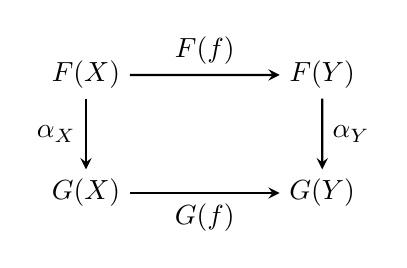
\begin{tikzpicture}[scale=1.5]
  \node (FX) at (0,1) {$F(X)$};
  \node (FY) at (2,1) {$F(Y)$};
  \node (GX) at (0,0) {$G(X)$};
  \node (GY) at (2,0) {$G(Y)$};
  
  \draw[->, >=stealth, thick] (FX) -- node[above] {$F(f)$} (FY);
  \draw[->, >=stealth, thick] (GX) -- node[below] {$G(f)$} (GY);
  \draw[->, >=stealth, thick] (FX) -- node[left] {$\alpha_X$} (GX);
  \draw[->, >=stealth, thick] (FY) -- node[right] {$\alpha_Y$} (GY);
\end{tikzpicture}
\end{center}
That is: $G(f) \circ \alpha_X = \alpha_Y \circ F(f)$.
If every component $\alpha_X$ is an isomorphism in $\mathcal{D}$, then $\alpha$ is a \newterm{natural isomorphism} ($F \cong G$).
\end{namedconcept}

\begin{enumerate}[label=(\alph*), leftmargin=*]
  \item Why can we not define a natural transformation between the identity functor $\text{Id}_{\mathbf{Vect}}$ and the single dual functor $(-)^*$? (Consider the variance of the two functors).
  \item Show how the evaluation map $\eta_V: V \to V^{**}$ resolves this: it forms a natural isomorphism between the identity functor $\text{Id}_{\mathbf{Vect}}$ and the double dual functor $(-)^{**}$.
\end{enumerate}

\newpage

\section{Part 3 --- Discovery}

\begin{discoverybox}
\textbf{What have we built?}

\textbf{First.} A category $\mathcal{C}$ abstracts mathematical systems into objects and morphisms (arrows) that compose associatively and possess identity arrows.

\textbf{Second.} Functors are mappings between categories that preserve structure. Covariant functors preserve the direction of morphisms, whereas contravariant functors reverse them.

\textbf{Third.} Natural transformations compare functors. A natural transformation $\alpha: F \Rightarrow G$ is a family of morphisms that commute with all morphism mappings between categories, formalizing basis-independence.

\textbf{Fourth.} The double dual mapping $\eta_V: V \to V^{**}$ is a natural isomorphism, proving that the equivalence of a finite-dimensional space to its double dual is coordinate-free (canonical).
\end{discoverybox}

\newpage

\section{Part 4 --- What This Is Called}

\begin{namedconcept}{Category Theory Parameters}
* **Morphism:** An arrow representing a structure-preserving relation between two objects in a category.
* **Functor:** A structure-preserving map between categories, mapping objects to objects and morphisms to morphisms.
* **Contravariant Functor:** A functor that reverses the composition order and direction of morphisms.
* **Natural Transformation:** A family of morphisms comparing two functors that commutes with all mapped morphisms.
* **Natural Isomorphism:** A natural transformation where every component morphic map is an isomorphism.
\end{namedconcept}

\newpage

\section{Part 5 --- Solved Exercises}

\begin{enumerate}[label=\textbf{E\arabic*.}]
  \item \textbf{Composition of Functors.}
  
        Prove that the composition of two covariant functors $F: \mathcal{C} \to \mathcal{D}$ and $G: \mathcal{D} \to \mathcal{E}$ is a covariant functor $G \circ F: \mathcal{C} \to \mathcal{E}$.
        
        \textbf{Solution:}
        To prove that $H = G \circ F$ is a covariant functor from $\mathcal{C} to \mathcal{E}$, we must verify that it satisfies the three functor axioms: object mapping, identity preservation, and composition preservation.
        
        1. **Object and Morphism Mappings:**
           * For any object $X \in \mathcal{C}$, $H(X) = G(F(X)) \in \mathcal{E}$, which is a valid object since $F(X) \in \mathcal{D}$ and $G$ maps objects of $\mathcal{D}$ to $\mathcal{E}$.
           * For any morphism $f: X \to Y$ in $\mathcal{C}$, $H(f) = G(F(f)): G(F(X)) \to G(F(Y))$ is a valid morphism in $\mathcal{E}$, since $F(f): F(X) \to F(Y)$ in $\mathcal{D}$ and $G$ maps morphisms of $\mathcal{D}$ to $\mathcal{E}$.
        
        2. **Identity Preservation:**
           For any object $X \in \mathcal{C}$:
           \[
             H(\text{id}_X) \;=\; G(F(\text{id}_X)).
           \]
           Since $F$ is a functor, it preserves identity: $F(\text{id}_X) = \text{id}_{F(X)}$.
           \[
             H(\text{id}_X) \;=\; G(\text{id}_{F(X)}).
           \]
           Since $G$ is a functor, it preserves identity:
           \[
             H(\text{id}_X) \;=\; \text{id}_{G(F(X))} \;=\; \text{id}_{H(X)}.
           \]
           Thus, identity is preserved.
        
        3. **Composition Preservation:**
           For any composed morphisms $f: X \to Y$ and $g: Y \to Z$ in $\mathcal{C}$:
           \[
             H(g \circ f) \;=\; G(F(g \circ f)).
           \]
           Since $F$ is a covariant functor:
           \[
             H(g \circ f) \;=\; G(F(g) \circ F(f)).
           \]
           Since $G$ is a covariant functor:
           \[
             H(g \circ f) \;=\; G(F(g)) \circ G(F(f)) \;=\; H(g) \circ H(f).
           \]
           Thus, composition is preserved.
        
        Therefore, $G \circ F$ is a covariant functor.
        
  \item \textbf{The Identity Natural Transformation.}
  
        Let $F: \mathcal{C} \to \mathcal{D}$ be a functor.
        Prove that there exists an identity natural transformation $\text{id}_F: F \Rightarrow F$ defined by $(\text{id}_F)_X = \text{id}_{F(X)}$ for all objects $X \in \mathcal{C}$.
        
        \textbf{Solution:}
        For $\text{id}_F$ to be a natural transformation, the naturality diagram must commute for any morphism $f: X \to Y$ in $\mathcal{C}$.
        The diagram for $\text{id}_F: F \Rightarrow F$ is:
        \begin{center}
        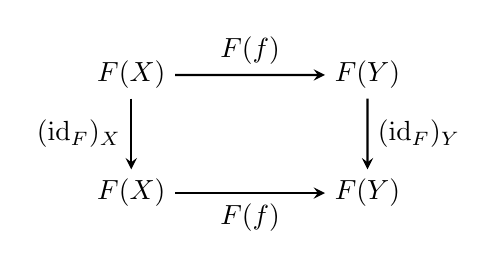
\begin{tikzpicture}[scale=1.5]
          \node (FX1) at (0,1) {$F(X)$};
          \node (FY1) at (2,1) {$F(Y)$};
          \node (FX2) at (0,0) {$F(X)$};
          \node (FY2) at (2,0) {$F(Y)$};
          
          \draw[->, >=stealth, thick] (FX1) -- node[above] {$F(f)$} (FY1);
          \draw[->, >=stealth, thick] (FX2) -- node[below] {$F(f)$} (FY2);
          \draw[->, >=stealth, thick] (FX1) -- node[left] {$(\text{id}_F)_X$} (FX2);
          \draw[->, >=stealth, thick] (FY1) -- node[right] {$(\text{id}_F)_Y$} (FY2);
        \end{tikzpicture}
        \end{center}
        The naturality condition requires:
        \[
          F(f) \circ (\text{id}_F)_X \;=\; (\text{id}_F)_Y \circ F(f).
        \]
        Substitute the defined components $(\text{id}_F)_X = \text{id}_{F(X)}$ and $(\text{id}_F)_Y = \text{id}_{F(Y)}$:
        \[
          F(f) \circ \text{id}_{F(X)} \;=\; \text{id}_{F(Y)} \circ F(f).
        \]
        By the identity axioms for morphisms in the category $\mathcal{D}$:
        * $F(f) \circ \text{id}_{F(X)} = F(f)$, since $F(f): F(X) \to F(Y)$.
        * $\text{id}_{F(Y)} \circ F(f) = F(f)$, since $F(f): F(X) \to F(Y)$.
        
        Both sides simplify to $F(f)$, so the equation holds:
        \[
          F(f) \;=\; F(f).
        \]
        Thus, the diagram commutes, proving that $\text{id}_F$ is a natural transformation.
\end{enumerate}

\newpage

\section{Part 6 --- Problems}

\begin{enumerate}[label=\textbf{P\arabic*.}]
  \item \textbf{The Opposite Category.}
  
        Let $\mathcal{C}$ be a category. We define the **opposite category** $\mathcal{C}^{\text{op}}$ as follows:
        * The objects of $\mathcal{C}^{\text{op}}$ are identical to the objects of $\mathcal{C}$.
        * The morphisms are reversed: $\text{Hom}_{\mathcal{C}^{\text{op}}}(A, B) = \text{Hom}_{\mathcal{C}}(B, A)$. That is, a morphism $f: A \to B$ in $\mathcal{C}^{\text{op}}$ corresponds to a morphism $f^{\text{op}}: B \to A$ in $\mathcal{C}$.
        
        \begin{enumerate}[label=(\alph*)]
          \item Prove that $\mathcal{C}^{\text{op}}$ satisfies the category axioms of identity and associativity.
          \item Let $F: \mathcal{C} \to \mathcal{D}$ be a contravariant functor.
                Show that $F$ can be formally represented as a *covariant* functor from the opposite category $\mathcal{C}^{\text{op}}$ to $\mathcal{D}$.
        \end{enumerate}

  \item \textbf{Forgetful and Free Functors.}
  
        The forgetful functor $U: \mathbf{Grp} \to \mathbf{Set}$ discards the group operation, mapping $(G, *)$ to its underlying set $G$.
        The **free functor** $F: \mathbf{Set} \to \mathbf{Grp}$ maps a set $S$ to the free group $F(S)$ generated by the elements of $S$.
        \begin{enumerate}[label=(\alph*)]
          \item Prove that the forgetful functor $U$ is a covariant functor.
          \item If $f: S \to T$ is a function between sets, describe how $F(f)$ maps generators to define a group homomorphism from $F(S) to F(T)$. Prove that $F$ is a covariant functor.
          \item Explain why the relationships between these two functors represent a fundamental duality: a map from a free group $F(S)$ to a group $G$ is uniquely determined by a function from the set $S$ to the set $U(G)$. (This is an **adjunction**, $F \dashv U$).
        \end{enumerate}
\end{enumerate}

\newpage

\section{Part 7 --- Deep Problems}

\begin{enumerate}[label=\textbf{D\arabic*.}]
  \item \textbf{Natural Isomorphism of the Double Dual.}
  
        Let $\mathbf{Vect}_{\text{fd}}$ be the category of finite-dimensional vector spaces over a field $K$.
        * Let $\text{Id}: \mathbf{Vect}_{\text{fd}} \to \mathbf{Vect}_{\text{fd}}$ be the identity functor.
        * Let $D: \mathbf{Vect}_{\text{fd}} \to \mathbf{Vect}_{\text{fd}}$ be the double dual functor, mapping a space $V$ to $V^{**}$ and a linear map $T: V \to W$ to $T^{**}: V^{**} \to W^{**}$.
        
        For each vector space $V$, define the evaluation mapping $\eta_V: V \to V^{**}$ by:
        \[
          \eta_V(v)(f) \;=\; f(v) \qquad \text{for all } v \in V \text{ and } f \in V^*.
        \]
        \begin{enumerate}[label=(\alph*)]
          \item Prove that $\eta_V$ is a linear mapping.
          \item Prove that if $\dim(V) < \infty$, the mapping $\eta_V$ is an isomorphism. \textit{Hint: Show that $\ker(\eta_V) = \{0\}$, which implies injectivity. Then use the dimension equivalence $\dim(V) = \dim(V^{**})$ to conclude bijection.}
          \item Prove that $\eta$ is a natural transformation by showing that for any linear map $T: V \to W$, the following diagram commutes:
          \begin{center}
          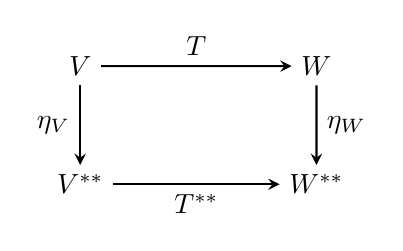
\begin{tikzpicture}[scale=1.5]
            \node (V) at (0,1) {$V$};
            \node (W) at (2,1) {$W$};
            \node (V2) at (0,0) {$V^{**}$};
            \node (W2) at (2,0) {$W^{**}$};
            
            \draw[->, >=stealth, thick] (V) -- node[above] {$T$} (W);
            \draw[->, >=stealth, thick] (V2) -- node[below] {$T^{**}$} (W2);
            \draw[->, >=stealth, thick] (V) -- node[left] {$\eta_V$} (V2);
            \draw[->, >=stealth, thick] (W) -- node[right] {$\eta_W$} (W2);
          \end{tikzpicture}
          \end{center}
          That is, prove $T^{**} \circ \eta_V = \eta_W \circ T$. This mathematically formalizes the basis-independence of the double-dual isomorphism.
        \end{enumerate}

  \item \textbf{Monoids and Groups as Single-Object Categories.}
  
        A **monoid** $(M, *, e)$ is a set with an associative binary operation and an identity element, but elements do not require inverses.
        \begin{enumerate}[label=(\alph*)]
          \item Show that a monoid $M$ is equivalent to a category $\mathcal{C}$ containing exactly one object, say $*$.
                Identify what the morphisms of $\mathcal{C}$ are, what composition represents, and what the identity morphism is.
          \item Show that a monoid homomorphism $\phi: M_1 \to M_2$ is equivalent to a covariant functor between their corresponding single-object categories.
          \item If a monoid is a category with one object, what is a group? Formulate a category-theoretic definition of a group.
        \end{enumerate}
\end{enumerate}

\newpage

\section{Part 8 --- Reflection}

\begin{reflectionbox}
\textbf{Conceptual Reflection}

Consider the following questions:
\begin{enumerate}
  \item **On Abstract Mappings:** Category theory has been jokingly called "generalized abstract nonsense" because it abstracts away all concrete details. Yet, it solved the decades-old confusion in linear algebra about "natural" vs "non-natural" mappings. Does abstraction clarify math by removing unnecessary details, or does it make it harder to visualize?
  \item **On the Geometry of Math:** By representing mathematical fields as categories and transitions as functors, category theory allows us to draw geometric diagrams (commuting squares and triangles) to prove algebraic theorems. What does this suggest about the connection between visual geometry and formal logic?
  \item **On Software Architecture:** In functional programming (like Haskell), types form a category where functions are morphisms, and generic type constructors (like `List` or `Maybe`) are functors. Why is the language of category theory so exceptionally suited for designing bug-free, highly abstract computer programs?
\end{enumerate}
\end{reflectionbox}

\medskip
\noindent\textbf{Looking ahead.}
Module~6.4 completes this journey by introducing **Monads and Universal Properties**. Having mastered categories, functors, and natural transformations, we will explore limits, colimits, and study the category-theoretic definition of a Monad, linking abstract algebra directly to functional computer science.

\vspace{1.4cm}
\begin{center}
{\color{NavyBlue}\rule{0.5\linewidth}{0.8pt}}\\[6pt]
{\small\color{NavyBlue}\textit{End of Journey 6, Module 6.3 --- Categories, Functors, and Natural Transformations}}\\[4pt]
{\small\color{NavyBlue}Continue to: \textbf{Module 6.4 --- Monads and Universal Properties}}\\[6pt]
{\color{NavyBlue}\rule{0.5\linewidth}{0.8pt}}
\end{center}

\end{document}
